\section{Задача маркетингової розвідки}
    \subsection{Огляд проблем МІС}
        \subsubsection{Основні поняття}
В ході аналізу проблемної області був складений глосарій:
            \begin{longEnumerate}
                \item Маркетинг --- це інститути та процеси, що створюють, доставляють та обмінюють пропозиції, що мають ціну для клієнтів, партнерів та суспільства в цілому\cite{kotler14}.  
                \item Маркетингова інформаційна система або МІС (англ. {\it marketing information system, MkIS}) --- це сукупність людей та систем, що виконують процедури збирання, сортування, аналізу та оцінки інформації для підтримки прийняття маркетингових рішень \cite{kotler14}. МІС може входити до складу більш загальної системи підтримки прийняття керівних рішень, EIS (англ. {\it executive information system})
                \item Маркетингове дослідження --- це систематичний збір та аналіз даних та висновків щодо конкретної ринкової ситуації, з якою зіткнулася компанія \cite{kotler14}.
                \item Маркетинговий канал --- це сукупність взаємопов’язаних організацій, що надають можливість використання та споживання різних товарів та послуг \cite{stern}.
% Маркетингова розвідка
            \end{longEnumerate}
        
        \subsubsection{Маркетингова розвідка як складова МІС}
        % навіщо потрібна маркетингова розвідка в МІС
        % хто займається, що на вході. 1 абзац.
Маркетингова інформаційна система складається з трьох частин \cite{kotler14}: внутрішній облік, маркетингові дослідження та розвідка. Основною частиною є маркетингові дослідження, а внутрішній облік та розвідка забезпечують дослідників точною, ретроспективною та щоденною інформацією про ринок та діяльність компанії. Збиранням внутрішньої ретроспективної інформації займаються системи внутрішнього обліку --- системи класів ERP та CRM. А збір щоденної, актуальної інформації з зовнішньої середи виконує маркетингова розвідка. За допомогою інтернету, засобів масової інформації, спеціалізованих агенств та звітності, комунікацій з клієнтами, в процесі розвідки збирається важлива інформація про стан ринку та ринкові тенденції. Наприклад, маркетингова розвідка може проінформувати дослідників, що згідно з новими статистичними звітами, змінився середній вік населення, а за допомогою інтернету визначити динаміку цін продуктів компаній-конкурентів.
 
            \begin{stdfigure}
                \includegraphics[width=7in]{images/mis_structure.png}
                \caption{Структура МІС}
                \label{fig:mis_structure}
            \end{stdfigure}    
   
        \subsubsection{Компоненти підсистеми маркетингової розвідки}
Формально, підстема маркетингової розвідки --- це процедури та джерела, які використовують маркетологи для збирання щоденної інформації про стан маркетингової середи\cite{kotler14}. Наразі, маркетингові інформаційні системи зосереджені на збиранні щоденної інформації та звітів про минулі періоди. Ця інформація допомагає дослідникам прогнозувати події на ринку та планувати власну маркетингову стратегію, але кінцева точність прогнозів сильно залежить від людського фактору, кваліфікації та досвіду аналітиків компанії.
 
Пропонується додати до підсистеми маркетингової розвідки складову (див. рис. \ref{fig:intelligence_scheme}), що буде автоматизувати процес прогнозування ринкової ситуації та надавати аналітикам перспективну інформацію. Автоматизація прогнозування дозволить скоротити витрати на маркетингові дослідження та збільшити точність прогнозів, що, в свою чергу, дозволить більш ефективно планувати діяльність компанії.

            \begin{stdfigure}
                \includegraphics[width=5in]{images/intelligence_scheme.png}
                \caption{Компоненти підсистеми маркетингової розвідки}
                \label{fig:intelligence_scheme}
            \end{stdfigure}    
  
    \subsection{Ділові ігри}
        \subsubsection{Поняття ділової гри}
Моделювання бізнес-систем є розповсюдженою практикою, що використовується в освіті та аналізі бізнес-процесів. Розглянемо один з методів моделювання: ділові ігри або бізнес-ігри (ці терміни взаємозамінні, від англ. {\it business game}). Ділова гра --- це процес послідовного або паралельного прийняття рішень учасниками ігри навколо деякої моделі бізнес-операції; ігри складаються з учасників, правил та ресурсів\cite{bg1, bg2}. Ігри можуть бути класифіковані за\cite{bg3}: наявністю конкуренції між учасниками, характером прийняття рішень (детермінований чи стохастичний), часовим інтервалом моделювання та ін.
        
        \subsubsection{Моделювання маркетингових каналів}
Структуру маркетингового каналу розглядають як керовану мережу систем, які працюють для досягнення спільної мети\cite{stern}: 
максимально прибутковий продаж товарів кінцевому споживачеві. До структури каналу входять чотири види учасників: виробники, дистриб’ютори (оптові торговці), рітейлери (магазини, супермаркети) та клієнти. Дистриб’ютори є посередниками між виробниками та рітейлерами, а рітейлери, в свою чергу, відділяють клієнтів від дистриб’юторів. Маркетинговий канал є конкурентною системою, бо його учасники можуть мати власні бізнес-цілі, що конфліктують з загальною метою маркетингового каналу. Приклад структури маркетингового каналу зображений на рис. \ref{fig:channel_structure}.

            \begin{stdfigure}
                \includegraphics[width=5in]{images/channel_structure.png}
                \caption{Приклад структури маркетингового каналу}
                \label{fig:channel_structure}
            \end{stdfigure}    

В каналі існує множина потоків, якими представляють процес функціонування каналу. Потік --- це сукупність функцій, які послідовно виконуються учасниками каналу, вони можуть бути прямими, зворотніми та двонаправленими; за допомогою потоків описують рух ресурсів по каналу. За Штерном, в маркетингових каналах є вісім універсальних потоків\cite{stern}: фізичне володіння товаром, право власності, просування, переговори, фінансування, ризик, розміщення замовлень, оплата.

Пропускна здатність каналу --- це максимальна кількість замовлень клієнтів, що може бути обслужена.

    \subsubsection{Постановка задачі моделювання}
%Вхід: структура каналу, набір параметрів поведінки гравців,     правила гри
%Вихід: дані щодо пропускної здатності каналу.
%На основі структури маркетингового каналу, параметрів поведінки гравців та правил ділової гри необхідно побудувати модель, що буде пронозувати поведінку реального маркетингового %каналу та надавати інформацію щодо його пропускної здатності. 

Моделювання --- це процесс побудови моделі для заміни досліджуємого об’єкту з метою дослідження його властивостей, прогнозування поведінки на основі властивостей моделі та характеристик її поведінки\cite{model}.
 
В цій роботі задача моделювання формулюється наступним чином: на основі структури маркетингового каналу, правил ділової гри та параметрів поведінки гравців необхідно побудувати модель маркетингового каналу, що буде прогнозувати його поведінку на вказаному проміжку часу. Метою моделювання є визначення пропускної здатності каналу.


    \subsection{Вимоги до ПЗ}
        \subsubsection{Функціональні вимоги}
        %TODO: use case, idef0
Функціональні вимоги описують поведінку системи та функції, що вона повинна виконувати. Для системи керування діловою грою <<Маркетинговий канал>> були визначені наступні функціональні вимоги:
            \begin{longEnumerate}
\item Система повинна підтримувати два типи користувачів (адміністратори та учасники) та надавати їм графічний інтерфейс для використання функціональних можливостей системи.
\item Адміністратор системи повинен мати можливість створювати нові ігри та видаляти їх. Для того, щоб створити гру, адміністратору необхідно ввести параметри гри (назва, дата початку та дата закінчення) та сформувати структуру маркетингового каналу, що буде моделюватися. 
\item Система повина надавати статистику функціонування каналу та визначати пропускну здатність каналу.
% Для створення маркетингового каналу, система повинна надавати можливість запрошувати учасників (за допомогою email), створювати модель учасника, видаляти учасників і моделі за потребою. 

            \begin{stdfigure}
                \includegraphics[width=7in]{images/uml_uc_admin.png}
                \caption{Діаграма варіантів використання для адміністратора}
                \label{fig:uml_uc_admin}
            \end{stdfigure}

% зробити ігри в множині
\item Адміністратор повинен мати можливість починати та зупиняти ігру, проглядати результати в реальному часі. Після запуску гри, система повинна почати імітацію діяльності маркетингового каналу та зберігати історію дій кожного з учасників.
% Після зупинки імітації, система повинна зробити знімок стану гри та зберегти його в вигляді, що дозволить імпортувати його до сховищ даних.
\item Учасники можуть відноситися до одного з чотирьох класів: виробник, дистриб’ютор, рітейлер, клієнт. Система повинна надати можливість визначити зв’язки між ними лише за наступними правилами: виробник може контактувати тільки з дистриб’юторами, дистриб’ютори можут контактувати тільки з виробниками та рітейлерами, рітейлери --- з дистриб’юторами та клієнтами, а клієнти --- тільки з дистриб’юторами.

            \begin{stdfigure}
                \includegraphics[width=5in]{images/uml_uc_players.png}
                \caption{Діаграма варіантів використанная для учасників гри}
                \label{fig:uml_uc_players}
            \end{stdfigure}
% [closed] TODO: несоответствие, тут: переглядати, робити замовленя у. В UML: вибирати контр-агента.
% Це нормально, в юз кейсах більш узагальнене формулювання.

% TODO: запитати про інформацію!
% Система повинна надавати  можливість зареєструватися учасникам, що були запрошені адміністратором для участі в грі.
\item  Система повинна надавати учасникам-виробникам можливість створювати товари у грі. Клєінти, дистриб’ютори та рітейлери повинні мати можливість робити замовлення: клієнти у рітейлерів, рітейлери у дистриб’юторів, дистриб’ютори у виробників. Система повинна надавати можливість виробникам, дистриб’юторам та рітейлерам обробляти вхідні замовлення.
      \end{longEnumerate}
        \subsubsection{Нефункціональні вимоги}
        % TODO: 6 критеріїв ISO. Перелічити!
Нефункціональні вимоги --- це вимоги, які визначають критерії роботи системи в цілому, а не окремі сценарії поведінки. Нефункціональні вимоги визначають системні властивості, такі як: функціональність, ефективність, зручність супроводу, розширюваність, надійність, середовищні фактори експлуатації. Для розроблюванної системи були розроблені наступні вимоги:
            \begin{longEnumerate}
\item В інтерфейсі користувача для учасників гри повинна будти одночасно відображена інформація про всіх доступних контрагентів та стан власних запасів учасника;
\item Модель учасника повинна бути реалізована таким чином, щоб зміна параметрів моделі не призводила до змін в програмному коді моделі; % TODO: ЩИТО?!
\item Обробка вхідного замовлення та замовлення як таке повинні проходити в рамках транзакцій.
            \end{longEnumerate}  
\subsection{Завдання на розробку ПЗ}
% TODO: несоответствие целей тут и целей моделирования. Вияснить.
% Исходя из постановкизадачи моделирования, делаем постановку задачи на  разработку.
Необхідно розробити програмний засіб для автоматизації процесу збирання перспективної інформації для систем маркетингової розвідки. На основі інформації про структуру маркетингового каналу та поведінку учасників розроблюваний програмний засіб повинен визначити пропускну здатність каналу за допомогою моделювання маркетингового каналу. Завдання на розробку проілюстроване на рис. \ref{fig:table}.
%TODO: прогнозувати попит та показники функціонування каналу
            \begin{stdfigure}
                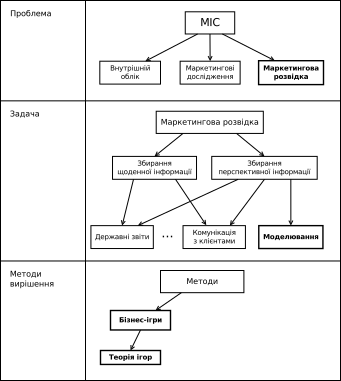
\includegraphics[width=7in]{images/table.png}
                \caption{Постановка задачі та методи її вирішення}
                \label{fig:table}
            \end{stdfigure}
% TODO: сделать сюда IDEF0?
